\documentclass[11pt,a4paper]{article}
% Muster-Entwurf Lösung Kurvendiskussion: FHR 2026 C, Aufgabe 1 a–f
% entlang ansaetze-kurvendiskussion (plan.md § 10 17.10. s, 18.10. a)
\usepackage{fontspec}
\setmainfont{DejaVu Sans}[Scale=0.9]
\usepackage{amsmath,amssymb}
\usepackage[left=16mm,right=16mm,top=12mm,bottom=12mm]{geometry}
\usepackage{xcolor,array,graphicx,tikz}
\definecolor{grau}{gray}{0.45}
\definecolor{linie}{gray}{0.75}
\pagestyle{empty}
\setlength{\parindent}{0pt}
\renewcommand{\arraystretch}{1.3}
\setlength{\tabcolsep}{4pt}
\newcommand{\g}[1]{{\small\color{grau}#1}}
\newcommand{\e}[1]{\boldsymbol{#1}}
% Teilaufgabe: Buchstabe, Stichworte aus der Ansatzsammlung (grau)
\newcommand{\teil}[2]{\par\vspace{7pt}{\color{linie}\hrule}\vspace{4pt}%
  \makebox[9mm][l]{\bfseries #1}\g{#2}\par\vspace{1pt}}
% Zeilen: links Zwischenergebnis, Mitte ⇒ bündig, rechts Folgerung
\newenvironment{kette}{\par\hspace*{9mm}%
  \begin{tabular}{@{}>{$}p{80mm}<{$}@{}>{$}c<{$}@{\ }>{$}l<{$}@{}}}%
  {\end{tabular}\par}
\newcommand{\dann}{\Rightarrow}

\begin{document}
\begin{center}
\includegraphics[page=2,height=0.93\textheight]{fhr26c.pdf}
\end{center}
\clearpage

{\large\bfseries 1 Differentialrechnung}\hfill\g{FHR 2026 C · Lösung}\par
\vspace{2pt}\hrule height 1.2pt\vspace{5pt}
$f(x)=-6x^5+18{,}75x^4+20x^3-90x^2$\par
\g{$x_N$ Nullstelle · $x_E$ Extremstelle · $x_W$ Wendestelle ·
$x_S$ Sattelstelle}

\teil{a)}{Verhalten im Unendlichen · Schnittpunkte mit den Achsen}
\begin{kette}
\text{höchste Potenz } -6x^5 & \dann &
  \lim\limits_{x\to-\infty}f(x)=+\infty,\
  \lim\limits_{x\to+\infty}f(x)=-\infty\\
 & \dann & \text{Abb. 2 und 4 fallen weg}\\
f(0)=0 & \dann & G_f \text{ verläuft durch } O
  \ \dann\ \text{Abb. 1 fällt weg}\\
 & \dann & \textbf{Abbildung 3}
\end{kette}

\teil{b)}{Symmetrie zum Ursprung · Nullstellen · Monotonie · Krümmung}
\begin{kette}
\text{(I) gerade Exponenten: } x^4,\ x^2 & \dann &
  \text{nicht punktsymmetrisch zu } O \ \dann\ \textbf{wahr}\\
\text{(II) } f(-3)\approx1626{,}75>0;\ f(-1)=-85{,}25<0 & \dann &
  x_N \text{ zwischen } -3 \text{ und } -1\\
 & \dann & S_x(x_N\,|\,0)\neq S_y(0\,|\,0)
  \ \dann\ \textbf{falsch}\\
\text{(III) 2 Extremstellen (e), 3 Wendestellen (f)} & \dann &
  \text{Krümmung wechselt öfter} \ \dann\ \textbf{wahr}
\end{kette}

\teil{c)}{Ableitung}
\begin{kette}
 & & \e{f'(x)=-30x^4+75x^3+60x^2-180x}\\
 & & \e{f''(x)=-120x^3+225x^2+120x-180}\\
 & & \e{f'''(x)=-360x^2+450x+120}
\end{kette}

\teil{d)}{Punktprobe · Tangente an der Stelle $x_0$}
\begin{kette}
f(3)=-209{,}25\neq-200 & \dann & A \notin G_f\\
f(-2)=-28 & \dann & \textbf{B liegt auf } \e{G_f}\\
m=f'(-2)=-480 & & \\
t(-2)=f(-2):\ -480\cdot(-2)+n=-28 & \dann & n=-988\\
 & \dann & \e{t(x)=-480x-988}
\end{kette}

\teil{e)}{Extremstellen · Hochpunkt · Tiefpunkt · Sattelstellen ·
Monotonie}
\begin{kette}
f'(-1{,}5)=0;\ f'(0)=0;\ f'(2)=0 & \dann &
  \text{Anstieg null an allen drei Stellen}\\[3pt]
f''(-1{,}5)=551{,}25>0;\ f(-1{,}5)\approx-129{,}52 & \dann &
  \textbf{Tiefpunkt } \e{T(-1{,}5\,|\,{-129{,}52})}\\
f''(0)=-180<0;\ f(0)=0 & \dann &
  \textbf{Hochpunkt } \e{H(0\,|\,0)}\\
f''(2)=0;\ f'''(2)=-420\neq0;\ f(2)=-92 & \dann &
  \textbf{Sattelpunkt } \e{S(2\,|\,{-92})}
\end{kette}
\vspace{2pt}
\hspace*{9mm}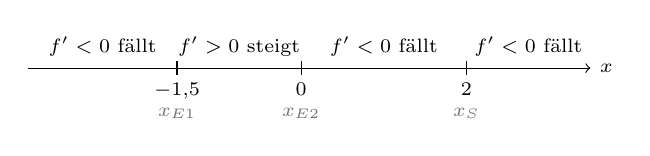
\begin{tikzpicture}[x=1.05cm,baseline=0]
  \draw[->,thin] (-3.3,0) -- (3.5,0) node[right,font=\scriptsize] {$x$};
  \foreach \p/\t/\n in {-1.5/{-1{,}5}/{x_{E1}},0/0/{x_{E2}},2/2/{x_S}}{
    \draw (\p,0.09)--(\p,-0.09);
    \node[below,font=\scriptsize] at (\p,-0.06) {$\t$};
    \node[below,font=\scriptsize,color=grau] at (\p,-0.38) {$\n$};}
  \node[above,font=\scriptsize] at (-2.4,0.02) {$f'<0$ fällt};
  \node[above,font=\scriptsize] at (-0.75,0.02) {$f'>0$ steigt};
  \node[above,font=\scriptsize] at (1,0.02) {$f'<0$ fällt};
  \node[above,font=\scriptsize] at (2.75,0.02) {$f'<0$ fällt};
\end{tikzpicture}
\begin{kette}
 & \dann & \textbf{fällt für } \e{x\le-1{,}5}\\
 & \dann & \textbf{steigt für } \e{-1{,}5\le x\le0}\\
 & \dann & \textbf{fällt für } \e{x\ge0}
\end{kette}

\teil{f)}{Wendestellen · Wendepunkte}
\begin{kette}
f''(2)=0 \ \text{\g{(ganzzahlig, geraten)}} & \dann & x_{W1}=2\\
f''(x):(x-2)=-120x^2-15x+90 \ \text{\g{(Division)}} & & \\
x^2+0{,}125x-0{,}75=0 \ \text{\g{(pq-Formel)}} & \dann &
  x_{W2}\approx-0{,}93;\ x_{W3}\approx0{,}81\\
f'''(-0{,}93)\approx-610{,}7;\ f'''(0{,}81)\approx248{,}9
  & \dann & \text{alle drei sind Wendestellen}\ \text{\g{($f'''(2)$ aus e)}}\\
 & \dann & \e{W_1(2\,|\,{-92})}\ \text{\g{(= S aus e)}}\\
 & & \e{W_2(-0{,}93\,|\,{-75{,}83})}\\
 & & \e{W_3(0{,}81\,|\,{-42{,}11})}
\end{kette}
\end{document}
